\chapter{\IfLanguageName{dutch}{Stand van zaken}{State of the art}}%
\label{ch:stand-van-zaken}

% Tip: Begin elk hoofdstuk met een paragraaf inleiding die beschrijft hoe
% dit hoofdstuk past binnen het geheel van de bachelorproef. Geef in het
% bijzonder aan wat de link is met het vorige en volgende hoofdstuk.

% Pas na deze inleidende paragraaf komt de eerste sectiehoofding.

%Dit hoofdstuk bevat je literatuurstudie. De inhoud gaat verder op de inleiding, maar zal het onderwerp van de bachelorproef *diepgaand* uitspitten. De bedoeling is dat de lezer na lezing van dit hoofdstuk helemaal op de hoogte is van de huidige stand van zaken (state-of-the-art) in het onderzoeksdomein. Iemand die niet vertrouwd is met het onderwerp, weet nu voldoende om de rest van het verhaal te kunnen volgen, zonder dat die er nog andere informatie moet over opzoeken \autocite{Pollefliet2011}.

%Je verwijst bij elke bewering die je doet, vakterm die je introduceert, enz.\ naar je bronnen. In \LaTeX{} kan dat met het commando \texttt{$\backslash${textcite\{\}}} of \texttt{$\backslash${autocite\{\}}}. Als argument van het commando geef je de ``sleutel'' van een ``record'' in een bibliografische databank in het Bib\LaTeX{}-formaat (een tekstbestand). Als je expliciet naar de auteur verwijst in de zin, gebruik je \texttt{$\backslash${}textcite\{\}}.
%Soms wil je de auteur niet expliciet vernoemen, dan gebruik je \texttt{$\backslash${}autocite\{\}}. In de volgende paragraaf een voorbeeld van elk.

%\textcite{Knuth1998} schreef een van de standaardwerken over sorteer- en zoekalgoritmen. Experten zijn het erover eens dat cloud computing een interessante opportuniteit vormen, zowel voor gebruikers als voor dienstverleners op vlak van informatietechnologie~\autocite{Creeger2009}.

%\lipsum[7-20]

Het onderzoek focused over fuctionele werken van de software voor tijdens de les zodat er een sneller installatie is waardoor er minder tijd moet gespenderen aan dit. Hier door zal ik mindere focusen over de precies werking van de verschillende software die niets te maken hebben met de installatie.

Maar zoals reeds vermeldt gaat dit onderzoek over het gebruik van containertechnologie om een gecombineerde installatie te doen van Hadoop, Spark en Kafka te automatiseren. Maar voor mensen die hier niet genoeg van afweten zal hier de nodige info worden vermeld om deze paper te bergrijpen.

\section{Containertechnologie}
A container technology is a lightweight, executable unit of software that packs up application code and dependencies such as binary code, libraries, and configuration files for easy deployment across different computing environments \autocite{Solarwinds2023}.
Meeste bekende gebruikte software's zijn Docker, CRI-O, rktlet, Containerd en runC

\subsection{Volume}
Volumes are the preferred mechanism for persisting data generated by and used by Docker containers.
The data is kept somewhere on storage attached to the host – often the local filesystem. The volume itself has a lifecycle that's longer than the container's, allowing it to persist until no longer needed. Volumes can be shared between containers. \autocite{Javatpoint2023}

Docker containers are used to run applications in an isolated environment. By default, all the changes inside the container are lost when the container stops. If we want to keep data between runs, Docker volumes and bind mounts can help. \autocite{Frieze2022}

\subsection{Docker}
Docker is a software platform that allows you to build, test, and deploy applications quickly. Docker packages software into standardized units called containers that have everything the software needs to run including libraries, system tools, code, and runtime. Using Docker, you can quickly deploy and scale applications into any environment and know your code will run. \autocite{AwsAmazon2023}

\subsubsection{Image}
A Docker container image is a lightweight, standalone, executable package of software that includes everything needed to run an application: code, runtime, system tools, system libraries and settings.\autocite{Docker2023a}

\subsubsection{Container}
Containers are an abstraction at the app layer that packages code and dependencies together. Multiple containers can run on the same machine and share the OS kernel with other containers, each running as isolated processes in user space. Containers take up less space than VMs (container images are typically tens of MBs in size), can handle more applications and require fewer VMs and Operating systems.\autocite{Docker2023a}

\subsection{Cluster}
A cluster in docker refers to multiple nodes joined. Containers are scheduled across the various nodes, and networking is configured with overlay networking to look similar to bridge networks to the containers, but across multiple nodes.\autocite{BMitch2019}

\subsection{Docker-compose}
Docker Compose is a tool that was developed to help define and share multi-container applications. With Compose, we can create a YAML file to define the services and with a single command, can spin everything up or tear it all down. \autocite{Docker2023}

\subsection{Kubernetes}
Kubernetes, or K8s for short, is an open-source container-orchestration tool designed by Google. It’s used for bundling and managing clusters of containerized applications — a process known as ‘orchestration’ in the computing world.
Kubernetes handles this changeover automatically and efficiently by restarting, replacing, and killing failed containers that don’t respond to a health check.\autocite{Guthrie2022}

\section{Virtual IT Company(VIC)}
VIC is een ``bedrijf'' in Hogent dat virtual machine's voorzie voor studenten en op aanvraag createn ze de contract bestlotende virtual machine('s) zodat zo iets niet op eigen computer moet draaien en/of installeren waardoor dit ook zal gebruikt worden voor als doel van dit onderzoek.

\subsection{Hypervisor}
A hypervisor, also known as a virtual machine monitor or VMM, is software that creates and runs virtual machines (VMs). A hypervisor allows one host computer to support multiple guest VMs by virtually sharing its resources, such as memory and processing.\autocite{VMware2023a}

\subsection{VMWare ESXi}
Discover a robust, bare-metal hypervisor that installs directly onto your physical server. With direct access to and control of underlying resources, VMware ESXi effectively partitions hardware to consolidate applications and cut costs. It’s the industry leader for efficient architecture, setting the standard for reliability, performance, and support.\autocite{VMware2023}

\subsection{vCenter}
vCenter Server is the centralized management utility for VMware, and is used to manage virtual machines, multiple ESXi hosts, and all dependent components from a single centralized location. VMware vMotion and svMotion require the use of vCenter and ESXi hosts.\autocite{Abbas2023}

\section{Hadoop}
The Apache Hadoop software library is a framework that allows for the distributed processing of large data sets across clusters of computers using simple programming models. It is designed to scale up from single servers to thousands of machines, each offering local computation and storage. Rather than rely on hardware to deliver high-availability, the library itself is designed to detect and handle failures at the application layer, so delivering a highly-available service on top of a cluster of computers, each of which may be prone to failures.\autocite{ASF2022}

\subsection{MapReduce}
At the crux of MapReduce are two functions: Map and Reduce. They are sequenced one after the other.
The Map function takes input from the disk as <key,value> pairs, processes them, and produces another set of intermediate <key,value> pairs as output.
The Reduce function also takes inputs as <key,value> pairs, and produces <key,value> pairs as output. \autocite{Talend2023}
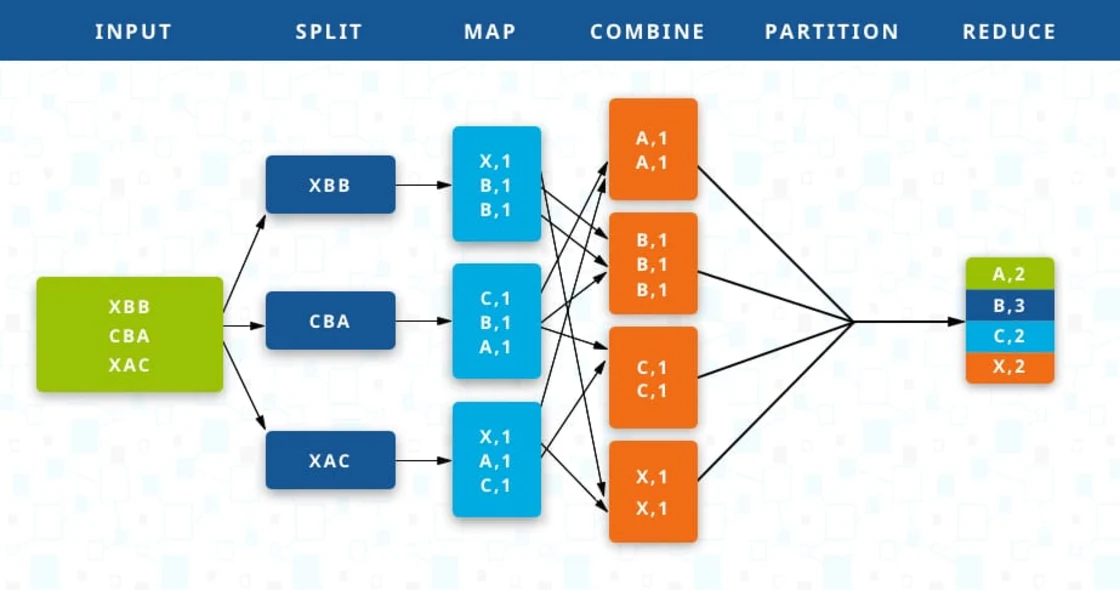
\includegraphics{mapreduce.png}

\subsection{HDFS}
The Hadoop Distributed File System (HDFS) is a distributed file system designed to run on
commodity hardware. It has many similarities with existing distributed file systems.
However, the differences from other distributed file systems are significant. HDFS is highly
fault-tolerant and is designed to be deployed on low-cost hardware. HDFS provides high
throughput access to application data and is suitable for applications that have large data sets.
HDFS relaxes a few POSIX requirements to enable streaming access to file system data.
HDFS was originally built as infrastructure for the Apache Nutch web search engine project.
HDFS is part of the Apache Hadoop Core project.\autocite{Borthakur2007a}

\section{Spark}
Apache Spark is an open-source, distributed processing system used for big data workloads. It utilizes in-memory caching, and optimized query execution for fast analytic queries against data of any size.
Spark was designed for fast, interactive computation that runs in memory, enabling machine learning to run quickly. The algorithms include the ability to do classification, regression, clustering, collaborative filtering, and pattern mining.\autocite{AwsAmazon2023a}

\subsection{Spark Core}
Spark Core is the underlying general execution engine for the Spark platform that all other functionality is built on top of. It provides in-memory computing capabilities to deliver speed, a generalized execution model to support a wide variety of applications, and Java, Scala, and Python APIs for ease of development.\autocite{databricks2023}

\subsection{Spark RDD}
Resilient Distributed Dataset (RDD) is the fundamental data structure of Spark. They are immutable Distributed collections of objects of any type. As the name suggests is a Resilient (Fault-tolerant) records of data that resides on multiple nodes.
\subsection{Spark SQL}
Many data scientists, analysts, and general business intelligence users rely on interactive SQL queries for exploring data. Spark SQL is a Spark module for structured data processing. It provides a programming abstraction called DataFrames and can also act as distributed SQL query engine. It enables unmodified Hadoop Hive queries to run up to 100x faster on existing deployments and data. It also provides powerful integration with the rest of the Spark ecosystem (e.g., integrating SQL query processing with machine learning).\autocite{databricks2023}

\subsection{Spark MLlib}
Machine learning has quickly emerged as a critical piece in mining Big Data for actionable insights. Built on top of Spark, MLlib is a scalable machine learning library that delivers both high-quality algorithms (e.g., multiple iterations to increase accuracy) and blazing speed (up to 100x faster than MapReduce). The library is usable in Java, Scala, and Python as part of Spark applications, so that you can include it in complete workflows.

\subsection{Spark GraphX}
Apache Spark's API for graphs and graph-parallel computation.
GraphX is a graph computation engine built on top of Spark that enables users to interactively build, transform and reason about graph structured data at scale. It comes complete with a library of common algorithms.\autocite{databricks2023}

\subsection{Spark Streaming}
Many applications need the ability to process and analyze not only batch data, but also streams of new data in real-time. Running on top of Spark, Spark Streaming enables powerful interactive and analytical applications across both streaming and historical data, while inheriting Spark’s ease of use and fault tolerance characteristics. It readily integrates with a wide variety of popular data sources, including HDFS, Flume, Kafka, and Twitter.\autocite{databricks2023}


\section{Kafka}
Apache Kafka is an open-source distributed event streaming platform used by thousands of companies for high-performance data pipelines, streaming analytics, data integration, and mission-critical applications.\autocite{ASF2022b}

Apache Kafka is a distributed data store optimized for ingesting and processing streaming data in real-time. Streaming data is data that is continuously generated by thousands of data sources, which typically send the data records in simultaneously. A streaming platform needs to handle this constant influx of data, and process the data sequentially and incrementally.
\autocite{AwsAmazon2023b}

\subsection{Broker}
A Kafka broker receives messages from producers and stores them on disk keyed by unique offset. A Kafka broker allows consumers to fetch messages by topic, partition and offset. Kafka brokers can create a Kafka cluster by sharing information between each other directly or indirectly using Zookeeper.\autocite{GitBook2023}

\subsection{Topic}
What are Apache Kafka Topics? Apache Kafka has a dedicated and fundamental unit for Event or Message organization, called Topics. In other words, Kafka Topics are Virtual Groups or Logs that hold messages and events in a logical order, allowing users to send and receive data between Kafka Servers with ease.\autocite{Ishwarya2022}

\subsection{Partitions}
What Is a Kafka Partition? In Apache Kafka, partitions are the main method of concurrency for topics. A topic, a dedicated location for events or messages, will be broken into multiple partitions among one or more Kafka brokers\autocite{Carder2022}

\subsection{Offset}
The consumer offset is a way of tracking the sequential order in which messages are received by Kafka topics. Keeping track of the offset, or position, is important for nearly all Kafka use cases and can be an absolute necessity in certain instances, such as financial services.\autocite{Dattell2023}


\section{Zookeeper}
\begin{Zookeeper}
    ZooKeeper is a centralized service for maintaining configuration information, naming, providing distributed synchronization, and providing group services. All of these kinds of services are used in some form or another by distributed applications. Each time they are implemented there is a lot of work that goes into fixing the bugs and race conditions that are inevitable. Because of the difficulty of implementing these kinds of services, applications initially usually skimp on them, which make them brittle in the presence of change and difficult to manage. Even when done correctly, different implementations of these services lead to management complexity when the applications are deployed.\autocite{ASF2023}
    
    What is ZooKeeper in Apache Kafka?
    Zookeeper is used for metadata management in the Kafka world. For example: Zookeeper keeps track of which brokers are part of the Kafka cluster. Zookeeper is used by Kafka brokers to determine which broker is the leader of a given partition and topic and perform leader elections. \autocite{Conduktor2023}
\end{Zookeeper}


Hadoop, Spark en Kafka worden al samen gebruikt volgens \textcite{Holmes2012}:
'In this situation, you'd use Kafka to both land data on Hadoop and provide a feed into a real-time data-streaming system such as Storm or Spark Streaming, which you could then use to perform near-real-time computations.' en \textcite{Leang2019}:
'one of the more significant findings to emerge from this study is that the integration of the Hadoop system especially Apache Kafka and Apache Spark enhances the performance and accuracy of data storing, processing, and securing in the manufacturing environment.'

Er is informatie te vinden over het gebruik van Docker om verschillende combinaties van 2 van de 3 frameworks te installeren maar niks over alle 3 samen, zeker niet met de requirements die wij willen onderzoeken. 

Zoals